\documentclass[letterpaper,12pt,oneside]{article}
\usepackage[top=1in, left=1.25in, right=1.25in, bottom=1in]{geometry}

\usepackage[T1]{fontenc}
\usepackage[utf8]{inputenc}
\usepackage[spanish,es-nodecimaldot,es-tabla]{babel}
\usepackage{caption, subcaption} %figuras
\usepackage{graphicx}
\usepackage{array}
\usepackage{imakeidx}
\usepackage{biblatex}
\addbibresource{bib/protocolo.bib}
\usepackage{float}
\usepackage{hyperref}
\usepackage{xurl}
\usepackage{amsmath} 

\graphicspath{{./figs/}}
\usepackage{setspace}
%\usepackage[round]{natbib}

\usepackage{tikz}
\usetikzlibrary{arrows.meta, positioning}

\begin{document}
%\frontmatter
\begin{titlepage}
		\setlength{\parindent}{0pt} \setlength{\parskip}{0pt}
	
		\begin{center}
			\vfill 
			
			\begin{minipage}{\textwidth}
				
				\newcolumntype{V}{>{\centering\arraybackslash} m{.17\textwidth} }
				\newcolumntype{C}{>{\centering\arraybackslash} m{.56\textwidth} }
				
				\begin{center}
					
\includegraphics[width=4.5cm]{escudoUNAM.jpg}	
				\end{center} 	
				\begin{center}
					\Huge\textbf{Universidad Nacional Autónoma de México}
				\end{center} 
				
			\end{minipage}
				
			\vfill
			
			\begin{minipage}{0.7\textwidth}
				\begin{center}
					\large Ingeniería en computación
				\end{center}
			\end{minipage}
			% 
			\begin{center}
				%\medskip \rule{.9\textwidth}{2pt}
				\vfill
				\large COMPILERS
				%{\Large \bfseries  \title   }
				
				%\medskip \rule{.9\textwidth}{2pt}
			\end{center}
			
			\begin{center}
				\vspace*{1cm}
				{\huge LEXER}\\
				\vspace*{1cm}
				
				%PRESENTA:\\ \medskip
				\begin{center}
					TEAM MEMBERS: \\
					\large
                    \item 423054589 - Arroyo Onofre Leonardo
                    \item 319061345 - Camacho Ignacio Violeta
                    \item 320047822 - Castañeda Luna Valeria
                    \item 423020441 - Martínez Pérez Diego Alexander
                    \item 320263635 - Ruiz Ramírez Santiago 
                    \item 320284858 - Saucedo Serralde Alejandra Melissa
                    
				\end{center}
				
				\bigskip
				
				GROUP: \#5\\
				%Coadvisors
				SEMESTER: \\
                2026-II
			\end{center}
			
			\vfill
			
			\begin{center}
				{México,CDMX. March 2026}\\
			\end{center}
			\cleardoublepage
		\end{center}
	\end{titlepage}
 
\tableofcontents
\clearpage
    
%\mainmatter

\section{Introduction} %
The challenge of this project is to implement a lexical analyzer capable of recognizing at least forty distinct tokens, including keywords, identifiers, operators, constants, strings, and punctuation marks, as well as to define a context-free grammar with left factoring for representative examples. 

Lexical analysis is the foundational stage of a compiler and its function is to transform the source code into a sequence of tokens that represent the minimal units of the language.
Providing a solution to this problem, that is, constructing a lexical analyzer, is necessary because without it the compiler would not be able to distinguish between keywords, identifiers, operators, constants, strings, or punctuation marks. The lexer organizes the code into recognizable components, detects early errors, and prepares the input for the subsequent stages of syntactic and semantic analysis. In this way, the compiler can correctly interpret the program, and the theoretical concepts of formal languages are translated into a practical and functional implementation.

By implementing the lexical analyzer, it is expected to obtain a functional lexer capable of recognizing forty distinct tokens, including keywords, identifiers, operators, constants, strings, and punctuation marks.
\begin{itemize}
    \item \textbf{Problem statement.} Before a program can be analyzed or executed by a compiler the source code must be transformed from a sequence of characters into meaningful elements, however, the raw text of a program does not initially contain an explicit structure that allows the compiler to interpret it.
    
    The problem addressed in this project is the design and implementation of a lexical analyzer capable of reading a source code input and identifying the basic tokens that compose it, these tokens include keywords, identifiers, operators, constants, literals, and punctuation symbols, additionally, the analyzer must count the total number of tokens detected in the input.
    
    By recognizing and classifying these elements the lexical analyzer provides the first structured representation of the program, which is necessary for further stages of the compilation process.
    
    \item \textbf{Motivation.} Lexical analysis is a fundamental stage in the compilation process because it allows the source code to be transformed into meaningful elements that can be processed by later stages of the compiler, without this step the compiler would not be able to distinguish between the different components of a program.
    
    The motivation for this project is to apply the theoretical concepts studied in class, particularly those related to lexical analysis and formal language processing in order to develop a functional lexical analyzer, by implementing a lexer it becomes possible to understand how source code is analyzed and structured during the early stages of compilation, as well as the importance of token recognition in the correct interpretation of a program.
    
    \item \textbf{Objective.} The objective of this project is to design and implement a lexical analyzer capable of reading a source code input and identifying the tokens that compose it, the system should recognize different token categories such as keywords, identifiers, operators, constants, literals, and punctuation symbols.

    Additionally the lexer must generate an output that displays the sequence of detected token types and the total number of tokens found in the input, by achieving this the project demonstrates the practical application of lexical analysis concepts and provides the first structured representation of the source code for further stages of compilation.
    
\end{itemize}

\section{Theoretical framework}
A compiler is a software system that is responsible for translating programs written in a high-level programming language into another language, typically machine code or an intermediate representation that can be executed by a computer, this translation is carried out through several stages among which lexical, syntactic, and semantic analysis are the most important, each stage processes the source program progressively until a representation is suitable for execution is obtained [1].

The first stage of this process is lexical analysis, performed by a component known as a lexical analyzer or lexer, this reads the source code as a stream of characters and groups them into meaningful units called tokens, these represent the smallest elements of a programming language, such as keywords, identifiers, operators, constants, literals, and punctuation symbols, during this stage the lexer may also remove elements that are not relevant for later stages such as whitespace and comments.[2]

A lexeme is the sequence of characters in the source code that matches the pattern of a token, for example, a reserved word like int, an identifier such as x, or a constant such as 10 are lexemes that correspond to different token categories, token recognition is commonly implemented using pattern matching techniques, such as regular expressions or finite automat, which allow the lexer to identify valid sequences of characters in the input program [3],[4].

Once the tokens are generated they are passed to the syntactic analysis phase, this stage verifies that the sequence of tokens follows the rules of the programming language, these rules are usually defined using Context-Free Grammars (CFGs), which describe the structure of valid sentences in the language using production rules [5].

A context-free grammar is typically defined as a tuple G=(V,T,P,S) where V is the set of non-terminal symbols, T is the set of terminal symbols, P is the set of production rules, and S is the start symbol, in order to simplify parsing and avoid ambiguities, grammar transformation techniques such as left factoring may be applied, left factoring restructures grammar rules that share common prefixes, making them more suitable for predictive parsing methods [5].

These theoretical concepts reviewed in class provided the foundation for the development of the lexical analyzer implemented in this project, which reads an input file, identifies lexemes, and classifies them into token categories for further processing in the compilation pipeline.


\section{Development}


First, the analyzer defines the lexical categories of the language. These categories include reserved words (keywords), identifiers, numeric constants, string literals, operators, punctuation symbols, comments, and whitespace. Each category represents a type of token that can appear in the source code.

Next, the analyzer prepares a collection of pattern definitions used to recognize each token type. These patterns are expressed as regular expressions, which allow the program to detect specific character sequences that correspond to valid tokens.

After defining the token patterns, the program reads the entire source file into memory. The analyzer then scans the input text sequentially, attempting to match one of the predefined patterns at the current position in the string. Whenever a pattern matches, the corresponding fragment of text is identified as a token and the scanning position moves forward.

This process continues until the end of the input is reached.

Once a fragment of text is recognized, the program determines the category of the token. Each recognized fragment is mapped into a higher-level classification used by the compiler.

For example:

\begin{itemize}
\item Words that match reserved language keywords are classified as keywords.
\item Character sequences that follow identifier naming rules but are not reserved words are classified as identifiers.
\item Numeric values such as integers, floating-point numbers, or hexadecimal values are classified as constants.
\item Text enclosed in quotation marks or single quotes is classified as a literal.
\item Mathematical or logical symbols are categorized as operators.
\item Symbols that structure the program, such as parentheses or commas, are treated as punctuation.
\end{itemize}

This classification step converts raw text fragments into standardized token types that the rest of the compiler can easily process.

An important responsibility of lexical analysis is handling elements that do not contribute to program semantics, such as whitespace and comments.

Whitespace characters (spaces, tabs, and line breaks) are used only to improve readability in source code. Similarly, comments provide explanations for human readers but are not relevant to the program's execution. For this reason, the analyzer detects these elements and simply ignores them instead of generating tokens.

By filtering out these non-significant components, the analyzer ensures that the resulting token stream contains only meaningful language constructs.

The analyzer operates using a sequential scanning strategy. At each step, it attempts to match the longest possible token that begins at the current position in the input string. Once a token is recognized, the scanning pointer advances by the length of that token.

This approach ensures that the analyzer processes the input deterministically and avoids overlapping matches. The program repeats this procedure until every character in the source file has been examined.

During the process, the analyzer records the type of each token found. At the end of the scan, the program outputs the sequence of token categories along with the total number of tokens identified.

To verify the correct behavior of the lexical analyzer, several tests were conducted using small fragments of C code as input. Each test evaluates whether the analyzer correctly identifies and classifies lexical elements such as keywords, identifiers, constants, operators, literals, and punctuation symbols. The tests also confirm that whitespace and comments are ignored during tokenization.

\subsection{Test 1}

\textbf{Input}

\begin{verbatim}
int a = 5;
\end{verbatim}

\textbf{Output}

\begin{verbatim}
keyword identifier operator constant punctuation
Total of tokens: 5
\end{verbatim}

\subsection{Test 2}

\textbf{Input}

\begin{verbatim}
float value = 3.14;
\end{verbatim}

\textbf{Output}

\begin{verbatim}
keyword identifier operator constant punctuation
Total of tokens: 5
\end{verbatim}

\subsection{Test 3}

\textbf{Input}

\begin{verbatim}
printf("Hello World");
\end{verbatim}

\textbf{Output}

\begin{verbatim}
keyword punctuation literal punctuation punctuation
Total of tokens: 5
\end{verbatim}

\subsection{Test 4}

\textbf{Input}

\begin{verbatim}
if (x >= 10) x++;
\end{verbatim}

\textbf{Output}

\begin{verbatim}
keyword punctuation identifier operator constant punctuation
identifier operator punctuation
Total of tokens: 9
\end{verbatim}

\subsection{Test 5}

\textbf{Input}

\begin{verbatim}
// comment
int x = 0;
\end{verbatim}

\textbf{Output}

\begin{verbatim}
keyword identifier operator constant punctuation
Total of tokens: 5
\end{verbatim}


\subsection{CFG with Left Factoring}
The following CFG represents the reading example int a = 5; used in test 1, the terminal symbols are in lowercase, while the non-terminal symbols are in capital letters.

\begin{align*}
S &\rightarrow \text{DECLARATION} \\
\text{DECLARATION} &\rightarrow \text{TYPE identifier DECLARATION}' \\
\text{DECLARATION}' &\rightarrow\;=\; \text{EXPRESSION} \;;\; \mid \;;\; \\
\text{EXPRESSION} &\rightarrow \text{constant} \mid \text{identifier} \\
\text{TYPE} &\rightarrow \texttt{int} \mid \texttt{float} \mid \texttt{char} \mid \texttt{double}
\end{align*}

The reason we decide to make it this way is because if we use for example.
\begin{align*}
\text{DECLARATION} &\rightarrow \text{TYPE identifier } =\; \text{EXPRESSION} \;;\; \mid \text{TYPE identifier }
\end{align*}
This would only bring us an ambiguous grammar due to a shared common prefix,  a parser would face a non-deterministic choice upon reading the TYPE and identifier tokens, it would not know which of the two production rules to choose without looking ahead
By applying left factoring to the DECLARATION' rule we isolated it and DECLARATION' was created, in order to handle the divergent suffixes. With his transformations the parser can determine exactly which production to apply.

\section{Results}

The following figures present the execution results of the lexical analyzer. Each example shows a screenshot of the input provided to the analyzer and the corresponding output produced by the program. These captures illustrate how the lexer classifies tokens according to the defined lexical categories while ignoring whitespace and comments.

\subsection{Test 1}

The following screenshots show the input provided to the lexical analyzer and the resulting token classification generated by the program.

\begin{figure}[H]
    \centering
    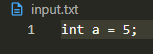
\includegraphics[width=0.5\linewidth]{results/input1.png}
    \caption{Input from Test 1}
    \label{fig:test1input}
\end{figure}

\begin{figure}[H]
    \centering
    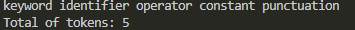
\includegraphics[width=0.75\linewidth]{results/output1.png}
    \caption{Output from Test 1}
    \label{fig:test1output}
\end{figure}

\subsection{Test 2}

The next images show the execution of the analyzer with the second input and the tokens identified in the output.

\begin{figure}[H]
    \centering
    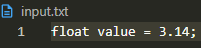
\includegraphics[width=0.5\linewidth]{results/input2.png}
    \caption{Input from Test 2}
    \label{fig:test2input}
\end{figure}

\begin{figure}[H]
    \centering
    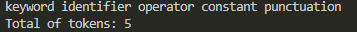
\includegraphics[width=0.75\linewidth]{results/output2.png}
    \caption{Output from Test 2}
    \label{fig:test2output}
\end{figure}

\subsection{Test 3}

These screenshots illustrate how the lexical analyzer processes literals and function calls within the source code.

\begin{figure}[H]
    \centering
    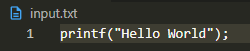
\includegraphics[width=0.5\linewidth]{results/input3.png}
    \caption{Input from Test 3}
    \label{fig:test3input}
\end{figure}

\begin{figure}[H]
    \centering
    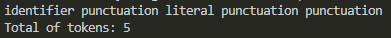
\includegraphics[width=0.75\linewidth]{results/output3.png}
    \caption{Output from Test 3}
    \label{fig:test3output}
\end{figure}

\subsection{Test 4}

The following figures show the analysis of conditional expressions and increment operators.

\begin{figure}[H]
    \centering
    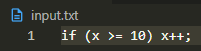
\includegraphics[width=0.5\linewidth]{results/input4.png}
    \caption{Input from Test 4}
    \label{fig:test4input}
\end{figure}

\begin{figure}[H]
    \centering
    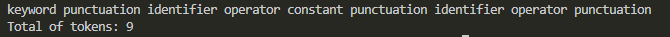
\includegraphics[width=0.75\linewidth]{results/output4.png}
    \caption{Output from Test 4}
    \label{fig:test4output}
\end{figure}

\subsection{Test 5}

Finally, the following screenshots demonstrate how the analyzer ignores comments and correctly processes the remaining tokens in the input.

\begin{figure}[H]
    \centering
    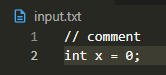
\includegraphics[width=0.5\linewidth]{results/input5.png}
    \caption{Input from Test 5}
    \label{fig:test5input}
\end{figure}

\begin{figure}[H]
    \centering
    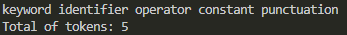
\includegraphics[width=0.75\linewidth]{results/output5.png}
    \caption{Output from Test 5}
    \label{fig:test5output}
\end{figure}



\subsection{CFG Step-by-step Derivation}

The following table shows how the grammar derives the input int a = 5;
step by step, applying the leftmost derivation:

\begin{table}[h]
\centering
\resizebox{\textwidth}{!}{
\begin{tabular}{|c|l|l|}
\hline
\textbf{Step} & \textbf{Sentential Form} & \textbf{Rule Applied} \\
\hline
1 & $S$ & Start symbol \\
\hline
2 & $\text{DECLARATION}$& $S \rightarrow \text{DECLARATION}$\\
\hline
3 & $\text{TYPE identifier DECLARATION}'$& $\text{DECLARATION} \rightarrow \text{TYPE identifier DECLARATION}'$\\
\hline
4 & $\texttt{int}\text{ identifier DECLARATION}'$& $\text{TYPE} \rightarrow \texttt{int}$\\
\hline
5& $\texttt{int identifier} = \text{EXPRESSION}\;;\;$& $\text{DECLARATION}' \rightarrow\; =\text{EXPRESSION}\;;\;$\\
\hline
6& $\texttt{int identifier} = \text{constant}\;;\;$& $\text{EXPRESSION} \rightarrow \text{constant}$\\\hline
 7& $\texttt{int a} = \text{constant}\;;\;$&$\text{identifier} \rightarrow \texttt{a}$ \\\hline
 8& $\texttt{int a = 5;}$ &$\text{constant} \rightarrow \texttt{5}$ \\\hline
\end{tabular}%
}
\caption{Leftmost derivation of \texttt{int a = 5;}}
\end{table}

\section{Conclusions}

The problem addressed in this project, transforming code into a structured sequence of tokens, required bridging the gap between the theoretical concepts studied in class and a functional software implementation, as this project demonstrates, this was made through design decisions like, how patterns are ordered, how conflicts between overlapping tokens are resolved, and how the boundary between scanning and classification is maintained consistently throughout the input.

The theoretical principles of regular expressions and pattern matching, initially seen and studied as abstract concepts, directly resulted in the creation of a reliable and predictable lexer. Any deviation from the theory leads to incorrect or inconsistent token recognition. The completeness of token coverage is not only  listing categories, but defining their boundaries precisely enough that no input sequence falls outside the expected classification.

The CFG checks if the tokens form a valid structure and left factoring makes explicit that validity alone is insufficient if the grammar cannot be parsed efficiently. All of these components seen previously together reflect what the problem statement anticipated, that lexical analysis is the first structured representation of a program, and that this must be correct, since this is what makes every subsequent stage of a compiler possible.

\section{References}

\noindent [1] IBM, ``What is a compiler?,'' \textit{IBM Think}, [Online].\\
Available: \url{https://www.ibm.com/mx-es/think/topics/compiler}. [Accessed: Mar. 2026].

\vspace{6pt}
\noindent [2] GeeksforGeeks, ``Introduction of Lexical Analysis,'' \textit{GeeksforGeeks}, [Online].\\
Available: \url{https://www.geeksforgeeks.org/compiler-design/introduction-of-lexical-analysis/}. [Accessed: Mar. 2026].

\vspace{6pt}
\noindent [3] GeeksforGeeks, ``Token, Patterns, and Lexemes,'' \textit{GeeksforGeeks}, [Online].\\
Available: \url{https://www.geeksforgeeks.org/compiler-design/token-patterns-and-lexems/}. [Accessed: Mar. 2026].

\vspace{6pt}
\noindent [4] TutorialsPoint, ``Compiler Design - Lexical Analysis,'' \textit{TutorialsPoint}, [Online].\\
Available: \url{https://www.tutorialspoint.com/compiler_design/compiler_design_lexical_analysis.htm}. [Accessed: Mar. 2026].

\vspace{6pt}
\noindent [5] GeeksforGeeks, ``What is Context-Free Grammar?,'' \textit{GeeksforGeeks}, [Online].\\
Available: \url{https://www.geeksforgeeks.org/theory-of-computation/what-is-context-free-grammar/}. [Accessed: Mar. 2026].
\end{document}

